\documentclass[10pt,a4paper]{article}
\usepackage{amsmath}
\usepackage{amssymb}
\usepackage{graphicx}
\usepackage{color}
\usepackage{fancyhdr}
\usepackage{fancyvrb}
\usepackage[margin=3.5cm]{geometry}
\usepackage{framed}
\usepackage{enumerate}
\usepackage{textcomp}
\def\ket#1{\left|#1\right\rangle}
\def\bra#1{\left\langle#1\right|}
\def\braket#1{\left\langle#1\right\rangle}
\usepackage{framed}

\definecolor{linkcol}{rgb}{0.0, 0.0, 0.5}
\usepackage[colorlinks=true,urlcolor=linkcol,citecolor=black,linkcolor=linkcol]{hyperref}

\renewcommand\thesection{2.\arabic{section}}
\renewcommand\thesubsection{\thesection.\arabic{subsection}}

\fancyhf{}
\lhead{\tiny Y.~D.~Chong (2016)}
\rhead{\scriptsize MH2801: Complex Methods for the Sciences}
\lfoot{}
\rfoot{\thepage}
\pagestyle{fancy}

\makeatletter
\def\PY@reset{\let\PY@it=\relax \let\PY@bf=\relax%
    \let\PY@ul=\relax \let\PY@tc=\relax%
    \let\PY@bc=\relax \let\PY@ff=\relax}
\def\PY@tok#1{\csname PY@tok@#1\endcsname}
\def\PY@toks#1+{\ifx\relax#1\empty\else%
    \PY@tok{#1}\expandafter\PY@toks\fi}
\def\PY@do#1{\PY@bc{\PY@tc{\PY@ul
\def\PYZdl{\char`\$}
\def\PYZhy{\char`\-}
\def\PYZsq{\char`\'}
\def\PYZdq{\char`\"}
\def\PYZti{\char`\~}

\begin{document}
\setcounter{page}{13}
\noindent
\underline{\textbf{\LARGE 2. Integrals}}
\vskip 0.1in

If we have a function $f(x)$ which is well-defined for some $a \le x
\le b$, its integral over those two values is defined as
\begin{equation}
\int_a^b dx\, f(x) \;=\; \lim_{N \rightarrow 0} \, \sum_{n=0}^{N} \Delta x\; f(x_n) \;\;\;\mathrm{where}\;\; x_n = a + n\Delta x, \;\; \Delta x \equiv \left(\frac{b-a}{N}\right).
\end{equation}
This is called a \textbf{definite integral}, and it represents the area
under the graph of $f(x)$ in the region between $x=a$ and $x=b$,
as shown in the figure below:

\begin{figure}[h]
  \centering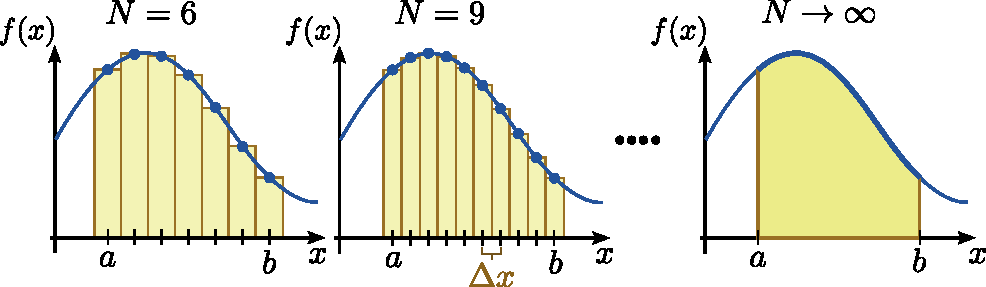
\includegraphics[width=0.9\textwidth]{definite_integral}
\end{figure}

\noindent
The interval between two fixed points, $a$ and $b$, is divided into
$N$ segments, of length $(b-a)/N$ each. Each term in the sum
represents the area of a rectangle. As $N\rightarrow \infty$, the sum
converges to the area under the curve.

For the purposes of dimensional analysis, an integral has the units of
the integrand times the units of $x$. This is easy to remember if you
think of $dx$ as a multiplicative factor with units of $x$.

From the defintion of the derivative, we can show that
\begin{equation}
  \frac{d}{db} \left[\int_a^b dx\; f(x)\right] = f(b), \quad \frac{d}{da} \left[\int_a^b dx\; f(x)\right] = -f(a).
\end{equation}
Hence, an integral is the ``inverse'' of a derivative operation. Notice
that the right-hand-side of the first equation does not involve $a$,
the opposite integral limit. Based on this, we can define an
\textbf{indefinite integral}, or \textbf{antiderivative}:
\begin{equation}
  \int^x dx' f(x') \equiv F(x) \;\;\mathrm{such}\;\mathrm{that}\;\; \frac{d}{dx}F(x) = f(x).
\end{equation}
Unlike a definite integral, an antiderivative is not unique, but is
only defined up to an additive constant, called an \textbf{integration
  constant}.

As you may recall from previous math classes, integration is much
harder than differentiation. Once you know how to differentiate a few
special functions, differentiating some combination of those functions
just involves a straightforward (though possibly tedious) application
of composition rules. By contrast, there is no general systematic
procedure for doing an integral symbolically. This is called the
\href{http://en.wikipedia.org/wiki/Antiderivative}{antiderivative
  problem}. Integration often involves making a series of inspired
choices, like guessing a solution and checking if its derivative gives
the desired integral expression. Some of the more commonly-used tricks
are summarized below.

\section{Integration by parts}

If the integrand consists of two factors, and you know the
antiderivative of one of the factors, you can ``integrate by parts''
to shift the derivative onto the other factor. Specifically,
\begin{equation}
  \int_a^b dx \; f(x) \, \frac{dg}{dx} \;=\; \Big[\,f(x)\,
    g(x)\,\Big]_a^b - \int_a^b \frac{df}{dx}\, g(x).
\end{equation}
The first term on the right hand side is a constant denoting
$[f(a)g(a) - f(b)g(b)]$. The second term is an integral, which might
be easier to do than the original integral. Judicious use of integration
by parts is a key step for solving many integrals.

For example, consider
\begin{equation}
  \int_a^b dx\; x \, e^{\gamma x}.
\end{equation}
The integrand consists of two factors, $x$ and $e^{\gamma x}$; we
happen to know the antiderivative of both factors. Integrating by
parts lets us replace one of these factors with its antiderivative,
while applying an additional derivative on the other factor. The smart
thing to do is to apply the derivative on the $x$ factor, and the
antiderivative on the $e^{\gamma x}$.  Then the first factor turns
into unity:
\begin{align}
  \int_a^b dx\; x\, e^{\gamma x} \;&=\; \left[\;x\, \frac{e^{\gamma x}}{\gamma}\, \right]_a^b - \int_a^b dx\; \frac{e^{\gamma x}}{\gamma} \\
  &=\; \left[\;x\, \frac{e^{\gamma x}}{\gamma} - \frac{e^{\gamma x}}{\gamma^2} \,\right]_a^b.
\end{align}
Whenever we finish doing an integral, it is good practice to
double-check the result by making sure the dimensions match up. Note
that $\gamma$ has units of inverse $x$, so the integral on the
left-hand side has units of $x^2$. The solution on the right hand side
has two terms, with units $x/\gamma$ and $1/\gamma^2$; both of these
are equivalent to units of $x^2$, which is what we need!

\section{Change of variables}
\label{change-of-variables}

Another useful technique for solving integrals is to change variables.
Consider the integral
\begin{equation}
  \int_0^\infty \frac{dx}{x^2 + 1}.
\end{equation}
We can solve this by making a change of variables $x = \tan(u)$. This
involves (i) replacing all occurences of $x$ in the integrand with
$\tan(u)$, (ii) replacing the integral limits, and (iii) replacing
$dx$ with $(dx/du) \, du = 1/[\cos(u)]^2 du$:
\begin{align}
  \int_0^\infty \frac{dx}{x^2 + 1} &= \int_0^{\pi/2} \frac{1}{[\tan(u)]^2 + 1} \cdot \frac{1}{[\cos(u)]^2} \; du \\ &= \int_0^{\pi/2} \frac{1}{[\sin(u)]^2 + [\cos(u)]^2} \; du.
\end{align}
Due to the Pythagorean theorem, the integrand reduces to 1, so
\begin{equation}
  \int_0^\infty \frac{dx}{x^2 + 1} = \int_0^{\pi/2} du = \frac{\pi}{2}.
\end{equation}
Clearly, this technique often requires some cleverness and/or
trial-and-error in choosing the right change of variables.

\section{The Gaussian integral}

Here's a famous integral:
\begin{equation}
  I(\gamma) = \int_{-\infty}^\infty \; e^{-\gamma x^2} \; dx.
  \label{gaussian}
\end{equation}
The integrand is called a \textbf{Gaussian} and is plotted below for
the case of $\gamma = 1$:

\begin{figure}[h]
  \centering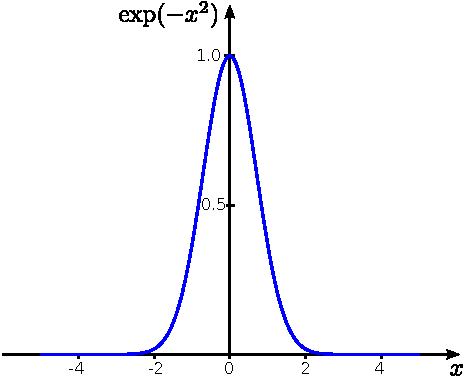
\includegraphics[width=0.46\textwidth]{gaussian}
\end{figure}

\noindent
The larger the value of $\gamma$, the more narrowly-peaked the curve.
Hence, the value of the definite integral depends on $\gamma$.

The integral was solved by
\href{http://en.wikipedia.org/wiki/Carl_Friedrich_Gauss}{Carl
  Friedrich Gauss} in a particularly brilliant way. If $I(\gamma)$
denote the value of the integral, $[I(\gamma)]^2$ is just two
independent copies of the integral, multiplied together:
\begin{equation}
  I^2(\gamma) = \left[\int_{-\infty}^\infty \; e^{-\gamma x^2} \; dx\right] \times \left[\int_{-\infty}^\infty \; e^{-\gamma y^2} \; dy\right].
\end{equation}
Note that in the second integral, we have changed the ``dummy'' label
$x$ (the integration variable) into $y$, to avoid ambiguity. Now, this
becomes a two-dimensional integral, taken over the entire 2D plane:
\begin{equation}
  I^2(\gamma) = \int_{-\infty}^\infty dx\, \int_{-\infty}^\infty dy \; e^{-\gamma (x^2+y^2)}.
\end{equation}
Next, we change from Cartesian to polar coordinates:
\begin{equation}
  I^2(\gamma) = \int_{0}^\infty dr\, r \int_{0}^{2\pi} d\phi \; e^{-\gamma r^2} = \left[ \int_{0}^\infty dr\, r \, e^{-\gamma r^2}\right] \times \left[\int_{0}^{2\pi} d\phi \right] = \frac{1}{2\gamma} \cdot 2\pi.
\end{equation}
Now, by taking the square root we arrive at the result
\begin{equation}
  I(\gamma) = \int_{-\infty}^\infty \; e^{-\gamma x^2} \; dx = \sqrt{\frac{\pi}{\gamma}}.
\end{equation}
One very interesting thing to notice about this result is that it
relates the two transcendental constants $e = 2.7182818285\dots$ and
$\pi = 3.141592654\dots$, by means of an integral. The appearance of
$\pi$ can be traced back to the use of polar coordinates to solve the
integral.

(As an aside, when studying the gamma function, we will come across
the fact that $\Gamma(1/2) = \pi$.  This is a very closely related
result which likewise relates $e$---which is incorporated into the
definition of the gamma function---and $\pi$.)

\section{Differentiating under the integral sign}
\label{differentiating-under-the-integral-sign}

In the previous section, we noted that if an integrand contains a
parameter (denoted $\gamma$) which is independent of the integration
variable (denoted $x$), then the definite integral can itself be
regarded as a function of $\gamma$. It can then be shown that taking
the derivative of the definite integral with respect to $\gamma$ is
equivalent to taking the `'partial derivative'' of the integrand:
\begin{equation}
  \frac{d}{d\gamma} \, \left[\int_a^b dx\; f(x,\gamma)\right] = \int_a^b dx \; \frac{\partial f}{\partial \gamma}(x,\gamma).
\end{equation}
This is called ``differentiating under the integral sign'', and was
originally invented by Gottfried Wilhelm Leibniz, one of the inventors
of calculus. It can be applied as a technique for solving integrals,
which was popularized by
\href{https://en.wikipedia.org/wiki/Richard_Feynman}{Richard Feynman}
in his book
\href{https://en.wikipedia.org/wiki/Surely_You\%27re_Joking,_Mr._Feynman!}{\emph{Surely You're Joking, Mr.~Feynman!}}.

Given a definite integral $I_0$, the technique proceeds as follows:
(i) come up with a way to generalize the integrand, by introducing a
parameter $\gamma$, such that the generalized integral becomes a
function $I(\gamma)$ which reduces to the original integral $I_0$ for
a particular parameter value, say $\gamma = \gamma_0$. Then, (ii)
differentiate under the integral sign. If you have chosen the
generalization right, the resulting integral will be easier to solve,
so (iii) solve the integral to obtain $I'(\gamma)$. Finally, (iv)
integrate this over $\gamma$ to obtain the desired integral
$I(\gamma)$, and evaluate it at $\gamma_0$ to obtain the desired
integral $I_0$.

An example will make the above procedure clearer. Consider the
integral
\begin{equation}
  \int_{0}^\infty dx \; \frac{\sin(x)}{x}.
\end{equation}
First, (i) we generalize the integral as follows (we'll soon see why):
\begin{equation}
  I(\gamma) = \int_{0}^\infty dx \; \frac{\sin(x)}{x}\, e^{-\gamma x}.
\end{equation}
The desired integral is $I(0)$. Next, (ii) differentiating under the
integral gives
\begin{equation}
  I'(\gamma) = - \int_{0}^\infty dx \; \sin(x)\, e^{-\gamma x}.
\end{equation}
Taking the partial derivative of the integrand with respect to
$\gamma$ brought down a factor of $-x$, cancelling out the troublesome
denominator. Now, (iii) we solve the new integral, which can be done
by integrating by parts twice:
\begin{align}
  I'(\gamma) &= \left[\cos(x)\,e^{-\gamma x}\right]_0^\infty + \gamma \int_{0}^\infty dx \; \cos(x)\, e^{-\gamma x} \\
  &= -1 + \gamma \left[\sin(x)\,e^{-\gamma x}\right]_0^\infty + \gamma^2 \int_{0}^\infty dx \; \sin(x)\, e^{-\gamma x}\\
  &= -1 - \gamma^2 I'(\gamma).
\end{align}
Hence,
\begin{equation}
  I'(\gamma) = - \frac{1}{1+\gamma^2}.
\end{equation}
Finally, (iv) we need to integrate this over $\gamma$.  But we already
know how to do this particular integral
\hyperref[change-of-variables]{in Section \ref{change-of-variables}},
and the result is
\begin{equation}
  I(\gamma) = A - \tan^{-1}(\gamma),
\end{equation}
where $A$ is a constant of integration. When $\gamma \rightarrow
\infty$, the integral must vanish, which implies that $A =
\tan^{-1}(+\infty) = \pi/2$. Finally, we arrive at the result
\begin{equation}
  \int_{0}^\infty dx \; \frac{\sin(x)}{x} = I(0) = \frac{\pi}{2}.
\end{equation}
It may seem to you that figuring out this sequence of steps would take
an large amount of ingenuity.  However, when we discuss contour
integration, we will see a more straightforward way to do this
particular integral.

\section{Exercises}
\label{exercises}

\begin{enumerate}
\item 
  Consider the step
function
\begin{equation}
  \Theta(x) = \left\{\begin{array}{ll} 1, &\;\;\;\textrm{for} \; x \ge 0\\ 0,&\;\;\; \textrm{otherwise.}\end{array}\right.
\end{equation}
Write down an expression for the antiderivative of $\Theta(x)$, and
sketch its graph.

\item
Show that
\begin{equation}\int_0^{2\pi} dx\, [\sin(x)]^2 =
\int_0^{2\pi} dx\, [\cos(x)]^2 = \pi.
\end{equation}

\item
Calculate the following definite integrals:
\begin{itemize}
\item
  $\displaystyle\int_{0}^\pi dx\; x^2 \sin(2x)$
\item
  $\displaystyle\int_{1}^\alpha dx\; x \ln(x)$
\item
  $\displaystyle\int_0^\infty dx\;e^{-\gamma x} \, \cos(x)$
\item
  $\displaystyle\int_0^\infty dx\;e^{-\gamma x} \, x \cos(x)$
\item
  $\displaystyle\int_{-\infty}^\infty dx\;e^{-\gamma |x|}$
\end{itemize}

\item
  By differentiating under the integral sign, solve
  \begin{equation}
    \int_0^1 dx\; \frac{x^2-1}{\ln(x)}.
  \end{equation}
  Hint: to generalize the integral, replace $x^2$ in the numerator
  with $x^\gamma$.
\end{enumerate}
    
    
\end{document}
